\documentclass[../main.tex]{subfiles}
%!TEX root = ./analysisArmFatigue.tex
\graphicspath {{../}}

\begin{document}
\section{Gondola Arm Fatigue Failure} \label{armFatigue}
The loading and unloading of the plastic gondola arm due to the reaction force of the keel on the gondola motor could potentially cause a fatigue failure. A paper on cyclic performance of Laser Sintered Nylon \cite{fatiguePlastic} was used to quantity the effects of fatigue on the plastic. Very little research has been done for fatigue failure of 3D printed material. The laser sintering process is similar to 3D printing in that it melts layers of plastic in succession to obtain complex geometries with no pre-existing tooling required. Because of this, the laser sintering process creates shear planes, much like those created in 3D printing. For this reason, the paper was as a basis for the fatigue analysis of the 3D printed part, as these shear planes are critical to the fatigue strength of the material. \\

The S-N curve shown in Figure \ref{fig:snCurve} was used to determine the maximum nominal stress that the gondola could take, thus defining the criteria for failure.

\begin{figure}[H]
	\centering
	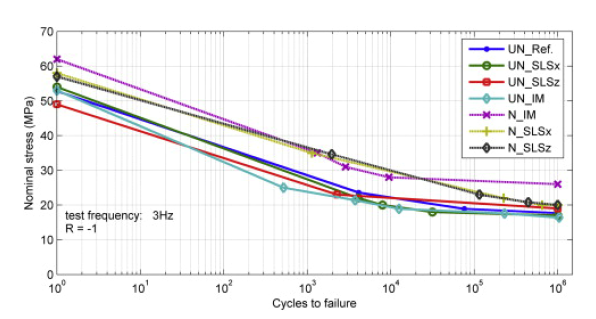
\includegraphics[width=.8\linewidth]{img/gondola/snCurve.PNG}
	\caption{S-N Curve for Laser Sintered Nylon \cite{fatiguePlastic}, Used to Determine the Fatigue Failure of the Gondola Body}
	\label{fig:snCurve}
\end{figure}

Assuming that the loading frequency is not higher than around 3hz, no appreciable heat is generated and thus the loading frequency should not affect the cycles to failure. Assuming SLS nylon, the maximum nominal stress for infinite life ($10^6$ cycles) is $17MPa$ Any higher and the part will fail after enough loading cycles.\\

To find the nominal stress, the amount of stress fluctuation which the gondola arm will sustain needs to be computed. For this, the lowest stress will be when the gondola is not moving, and is only loaded by the weight of the gondola itself. The highest stress will be when the gondola motor is on at full force, at the worst case scenario \textbf{DESCRIBED HERE} bending the gondola arm. These both conditions are computed using \textbf{ISAAKS SHIT HERE}, and two values of $F_{NB}$ are found. The difference between the two is the fluctuation of stress.
\begin{equation}
	\sigma_{worst}= \underbrace{\left[\left(\dfrac{F_{NB_{z}}}{A}\right)\hat{k} + \left(\dfrac{F_{NB_{y}}l_{arm}c}{I}  + \dfrac{M_{NB}c}{I} \right) \hat{j}\right]}_\text{Worst Case $F_{NB}$}, \sigma_{best} = \underbrace{\left[\left(\dfrac{F_{NB_{z}}}{A}\right)\hat{k} + \left(\dfrac{F_{NB_{y}}l_{arm}c}{I}  + \dfrac{M_{NB}c}{I} \right) \hat{j}\right]}_\text{Best Case $F_{NB}$}
\end{equation}

The principle stress for each case $\sigma _a$ is found, and the difference is computed to get the nominal strength, which must be less than $17MPa$. Therefore the optimized equation is:

\begin{equation}
	17Mpa \geq \left|\sigma _{a_{best}}-\sigma _{a_{worst}}\right|
\end{equation} 

\end{document}